% Az agent-alapú rendszer felépítése (5. fejezet). Fordítás: pdflatex agent_architektura.tex
\documentclass[tikz,border=4pt]{standalone}
\usepackage[utf8]{inputenc}
\usepackage[T1]{fontenc}
\usepackage{times}
\usetikzlibrary{positioning,arrows.meta,shapes.geometric,fit,backgrounds,calc}
\definecolor{det}{HTML}{1D294D}
\definecolor{detbg}{HTML}{E6ECF7}
\definecolor{llm}{HTML}{B7791F}
\definecolor{llmbg}{HTML}{FEEFCF}
\definecolor{dat}{HTML}{4A5568}
\definecolor{datbg}{HTML}{F3F4F7}
\begin{document}
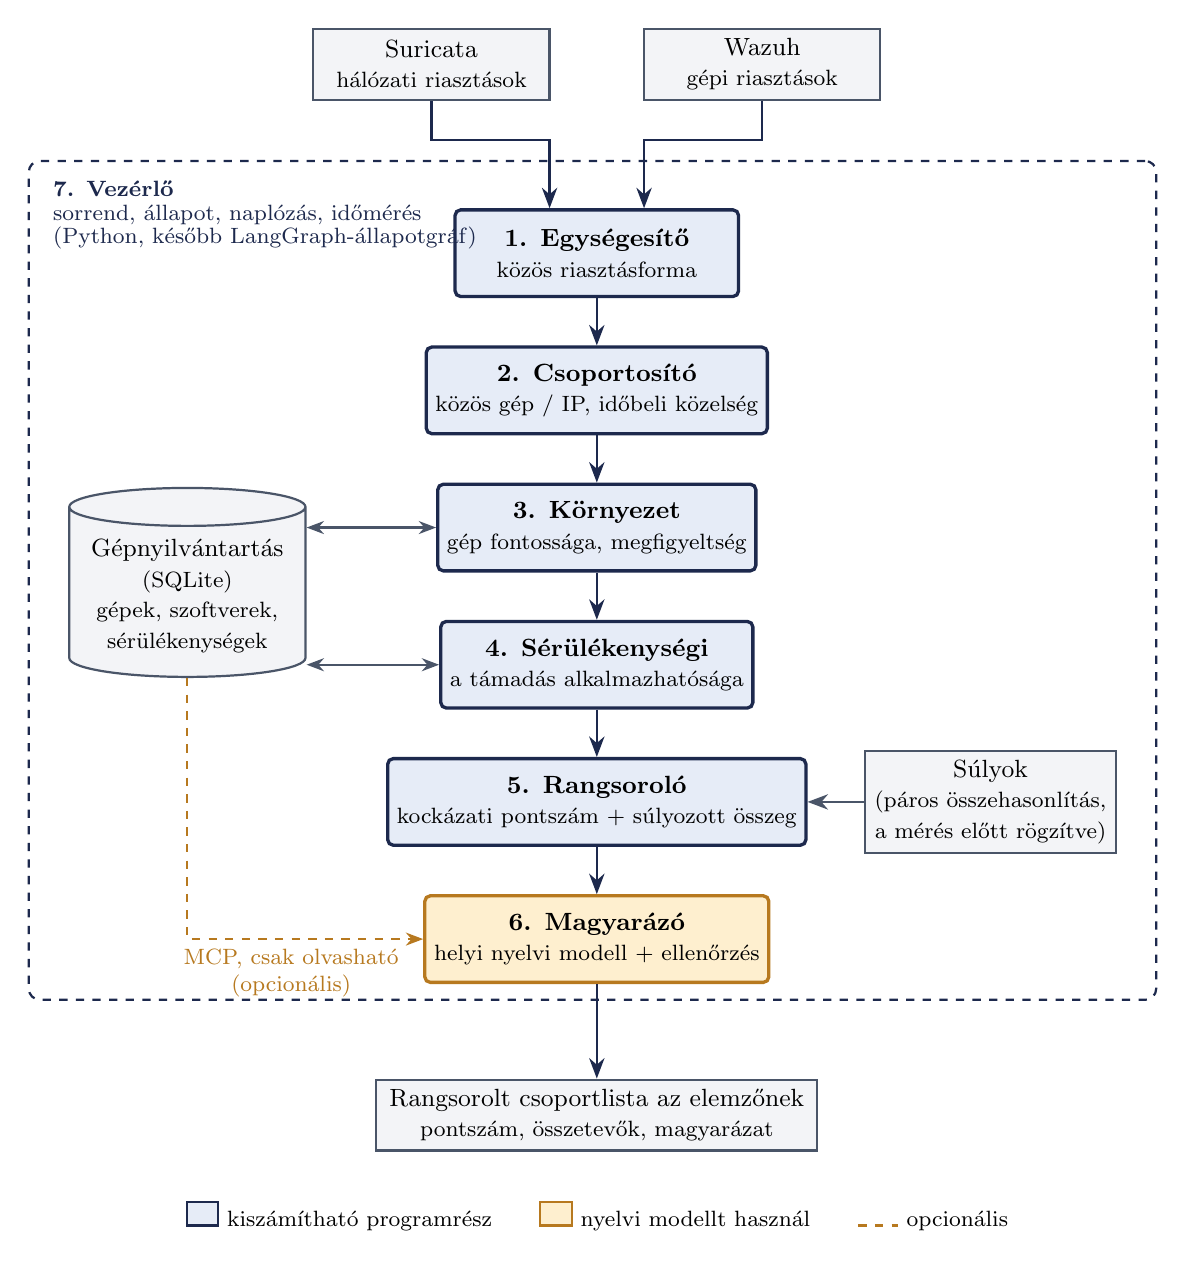
\begin{tikzpicture}[
  font=\small,
  node distance=6mm and 8mm,
  agent/.style={draw=det, fill=detbg, very thick, rounded corners=2pt, minimum width=36mm,
                minimum height=11mm, align=center},
  llmagent/.style={agent, draw=llm, fill=llmbg},
  src/.style={draw=dat, fill=datbg, thick, minimum width=30mm, minimum height=9mm, align=center},
  db/.style={cylinder, shape border rotate=90, aspect=0.18, draw=dat, fill=datbg, thick,
             minimum width=30mm, minimum height=13mm, align=center},
  flow/.style={-{Stealth[length=2.6mm]}, thick, draw=det},
  look/.style={{Stealth[length=2.2mm]}-{Stealth[length=2.2mm]}, thick, draw=dat},
  opt/.style={-{Stealth[length=2.2mm]}, thick, dashed, draw=llm},
]
% források
\node[src] (sur) at (-21mm,0) {Suricata\\\footnotesize hálózati riasztások};
\node[src] (waz) at (21mm,0) {Wazuh\\\footnotesize gépi riasztások};
% fő folyam (egy oszlop)
\node[agent] (norm) at (0,-24mm) {\textbf{1. Egységesítő}\\\footnotesize közös riasztásforma};
\node[agent, below=of norm] (grp) {\textbf{2. Csoportosító}\\\footnotesize közös gép / IP, időbeli közelség};
\node[agent, below=of grp] (ctx) {\textbf{3. Környezet}\\\footnotesize gép fontossága, megfigyeltség};
\node[agent, below=of ctx] (vul) {\textbf{4. Sérülékenységi}\\\footnotesize a támadás alkalmazhatósága};
\node[agent, below=of vul] (rank) {\textbf{5. Rangsoroló}\\\footnotesize kockázati pontszám + súlyozott összeg};
\node[llmagent, below=of rank] (expl) {\textbf{6. Magyarázó}\\\footnotesize helyi nyelvi modell + ellenőrzés};
\node[src, below=12mm of expl, minimum width=56mm] (out) {Rangsorolt csoportlista az elemzőnek\\\footnotesize pontszám, összetevők, magyarázat};
% adatok oldalt
\node[db, minimum height=24mm] (inv) at ($(ctx)!0.5!(vul)+(-52mm,0)$) {Gépnyilvántartás\\\footnotesize (SQLite)\\\footnotesize gépek, szoftverek,\\\footnotesize sérülékenységek};
\node[src, minimum width=28mm] (w) at ($(rank)+(50mm,0)$) {Súlyok\\\footnotesize (páros összehasonlítás,\\\footnotesize a mérés előtt rögzítve)};
% nyilak
\draw[flow] (sur.south) -- ++(0,-5mm) -| ([xshift=-6mm]norm.north);
\draw[flow] (waz.south) -- ++(0,-5mm) -| ([xshift=6mm]norm.north);
\draw[flow] (norm) -- (grp);
\draw[flow] (grp) -- (ctx);
\draw[flow] (ctx) -- (vul);
\draw[flow] (vul) -- (rank);
\draw[flow] (rank) -- (expl);
\draw[flow] (expl) -- (out);
\draw[look] (inv.east |- ctx.west) -- (ctx.west);
\draw[look] (inv.east |- vul.west) -- (vul.west);
\draw[flow, draw=dat] (w) -- (rank);
\draw[opt] (inv.south) |- node[pos=0.72, below, font=\footnotesize, text=llm, align=center] {MCP, csak olvasható\\(opcionális)} (expl.west);
% vezérlő keret
\begin{scope}[on background layer]
  \node[draw=det, thick, dashed, rounded corners=4pt, fill=white,
        fit=(norm)(grp)(ctx)(vul)(rank)(expl)(inv)(w), inner xsep=5mm, inner ysep=4mm,
        yshift=2mm] (ctrl) {};
\end{scope}
\node[anchor=north west, font=\footnotesize\bfseries, text=det, align=left]
  at ([xshift=2mm,yshift=-1.5mm]ctrl.north west)
  {7. Vezérlő\\[-1pt]\mdseries sorrend, állapot, naplózás, időmérés\\[-1pt]\mdseries (Python, később LangGraph-állapotgráf)};
% jelmagyarázat
\node[below=5mm of out, font=\footnotesize, align=center] (leg) {
  \tikz\node[draw=det, fill=detbg, thick, minimum width=4mm, minimum height=3mm]{}; kiszámítható programrész\qquad
  \tikz\node[draw=llm, fill=llmbg, thick, minimum width=4mm, minimum height=3mm]{}; nyelvi modellt használ\qquad
  \tikz\draw[dashed, thick, draw=llm] (0,0) -- (5mm,0); opcionális};
\end{tikzpicture}
\end{document}
